\label{multiProt}
The focus in this section is on interactions obtained from setup 4 occurring between multiple FAK molecules. At this point, we want to remind the reader that the used protein structure lacks the FAT domain, which is in full length FAK connected to the kinase via a linker region. This might have a significant effect on clustering processes.
\subsection{Dimerization of FAK}
\label{mult:dimers}
First, we want to investigate interactions between two FAK molecules. To this end, we filtered the dataset for interactions in which both partners have exactly one neighbour (dimers). It turns out that FERM-kinase dimers (type 3 neighbours) occur the most, followed by FERM-FERM dimers (type 1 neighbours). Probably, this does not reflect an energetic preference but is rather attributed to the initial biased preference of type 1 interactions (see \autoref{methods:contactana}). Regarding our observations, the number of encounters of FERM-FERM dimers plus the number of encounters of kinase-kinase dimers is, indeed, very similar to the number of encounters of FERM-kinase dimers. Actually, it is difficult to retrieve the energetic preference of the dimerization-type in \martini{}. Since two proteins can only interact within the cut-off radius of long range interactions, the proteins forming a dimer are already very close before starting to interact and might can not adjust their orientations.\\
\\
Because FERM-FERM dimers have been experimentally investigated by \textcite{fakdimers}, a short comparison between the obtained results and the experimental findings follows. For this purpose, we chose the FERM-FERM dimer with the longest lasting time as a representative example.\\
The contact map of the interaction surface is shown in \autoref{mult:fermfermcontact}. From this, the importance of residue \acid{W}{266} can be confirmed (orange region). Beside this, also the residues \acid{Y}{282} to \acid{K}{286} (green region) and \acid{T}{291} to \acid{A}{294} (red region) appear as important actors at the interaction surface since they interact with \acid{W}{266} and among each other. However, the RMSF value of these distances is larger than for the pairs involving \acid{W}{266}.\\
At this point, it has to be remarked that other FERM-FERM dimers in the simulation also show contacts between F1 and F3. Yet, since these contacts are not visible in other samples (e.g. the chosen one), they are not presented here.\\
Comparing the FERM-kinase interfaces of the involved proteins to FAK-MEM, we noticed a decrease of the inter residue distances by ca. $0.2\,\si{\nano\metre}$. This can be attributed to the fact that FERM-FERM dimerisation requires an uplift of F3, because the interaction interface points towards the membrane in FAK-MEM. Since the FERM domain is anchored on the membrane via the basic patch, this would push the kinase partly into the membrane (see \autoref{mult:fermferm_sketch}). Therefore, a force is acting on the kinase, which is a possible reason for the observed closure.
%
%
%
\begin{figure}[h]
	\subcaptionbox{\label{mult:fermferm_sketch}}[0.49\textwidth]{
		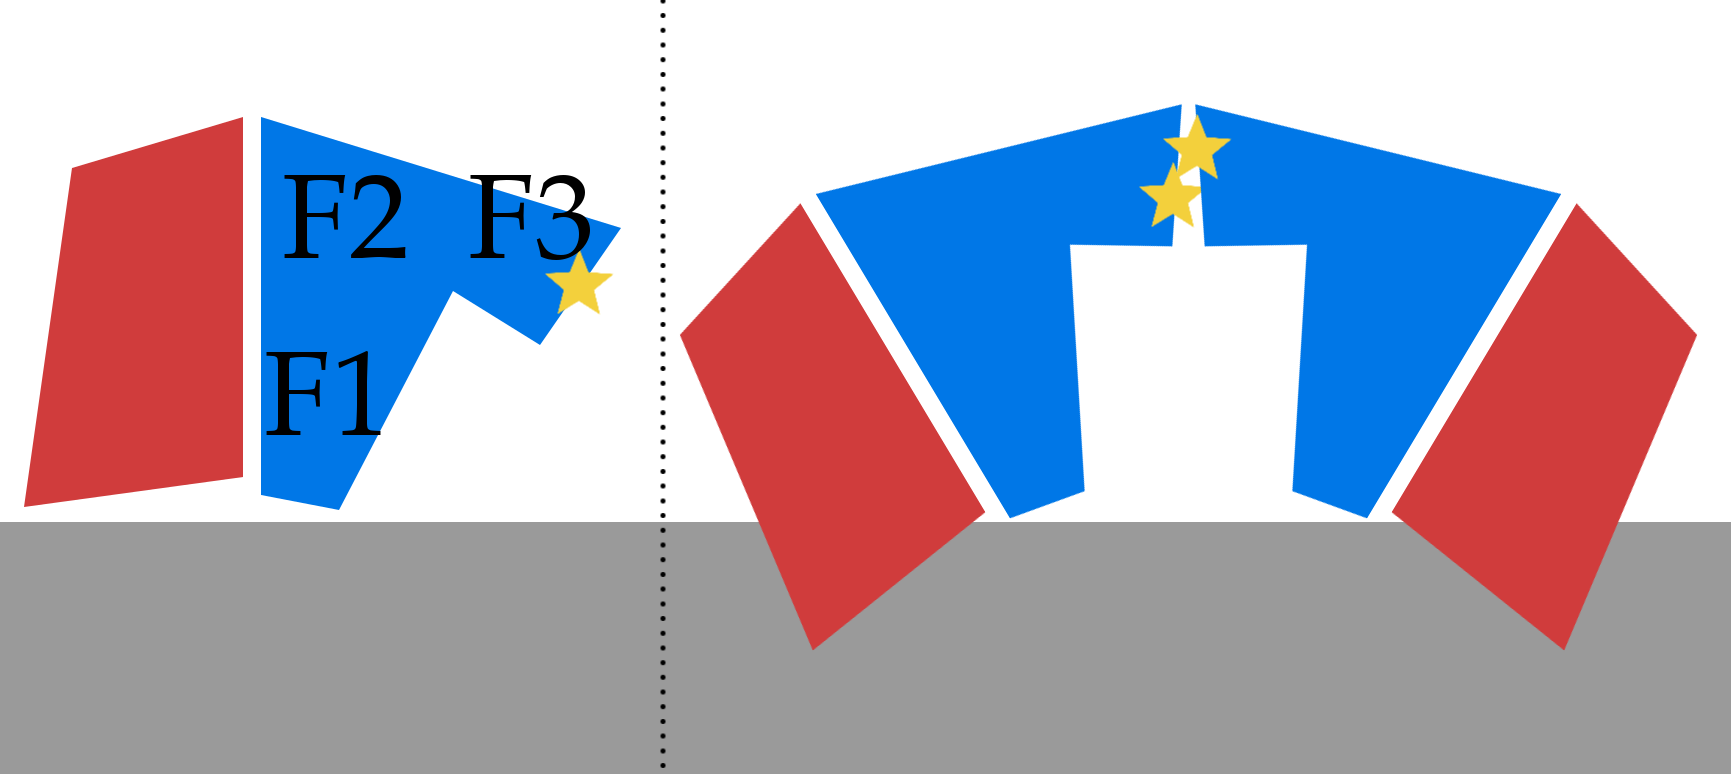
\includegraphics[height=3cm]{figures/results/fermfermdimer_sketch}
		\vspace{1.5cm}
	}\hfill%
	\subcaptionbox{\label{mult:fermfermcontact}}[0.5\textwidth]{
		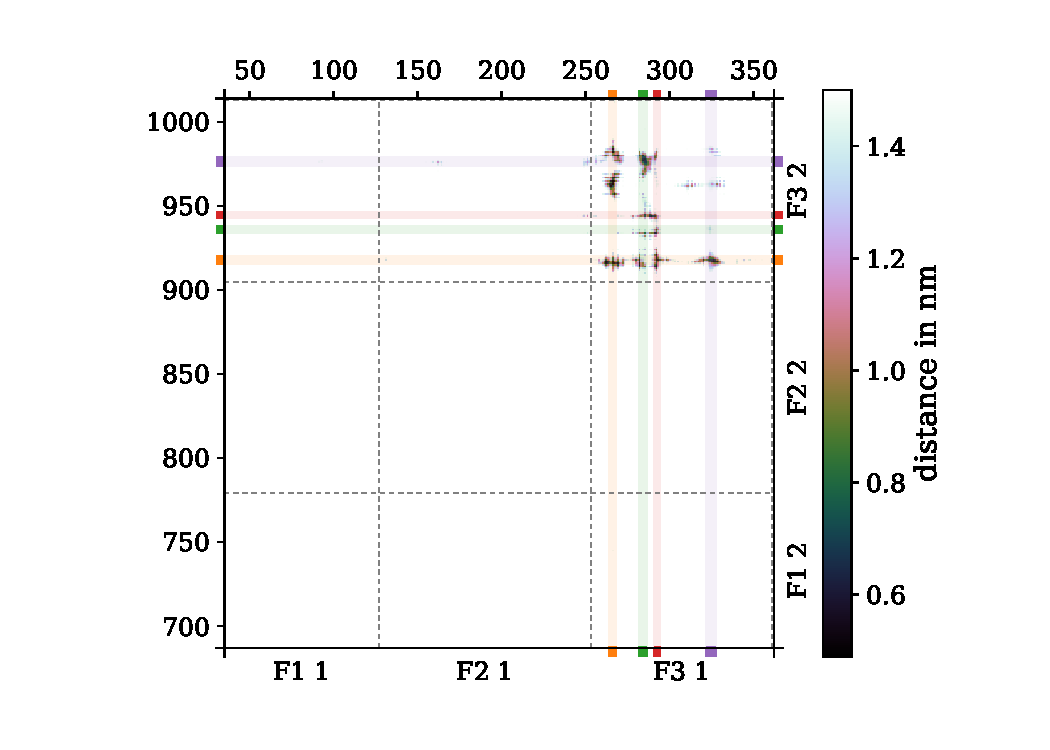
\includegraphics[height=6cm]{figures/results/fermferminterface}
	}
	\nicecaption{FERM-FERM dimers}{(\subref{mult:fermferm_sketch}): Sketch of FERM-FERM dimer. In FAK-MEM (left) the interaction site points to the membrane. Therefore, an uplift of F3 is required for dimerization (right), which pushes the kinase into the membrane. \acid{W}{266} is marked with a star. (\subref{mult:fermfermcontact}):  Contact map of the interaction site between the two FERM domains (only F3 is shown). \acid{W}{266} (orange) forms a lot of contacts with the neighbouring FAK molecule. In addition, the regions around \acid{Y}{282} (green) and \acid{H}{292} (red) are important contributors.}
	\label{mult:fermferm}
\end{figure}
%
%
%
\subsection{FAK clusters}
\label{mult:oligs}
The characterisation of the emerged FAK clusters is very difficult as they differ a lot in size and shape. The largest cluster observed in setup 4 has a size of 21 proteins, while there are other proteins, which did not join any cluster at all. Present shapes of the clusters include long chains as well as ring-like conformations or just agglomerations (see \autoref{clust:3d}).\\
%
%
%
\begin{figure}[hb]
	\subcaptionbox{\label{clust:3d_chain}}[0.32\textwidth]{
		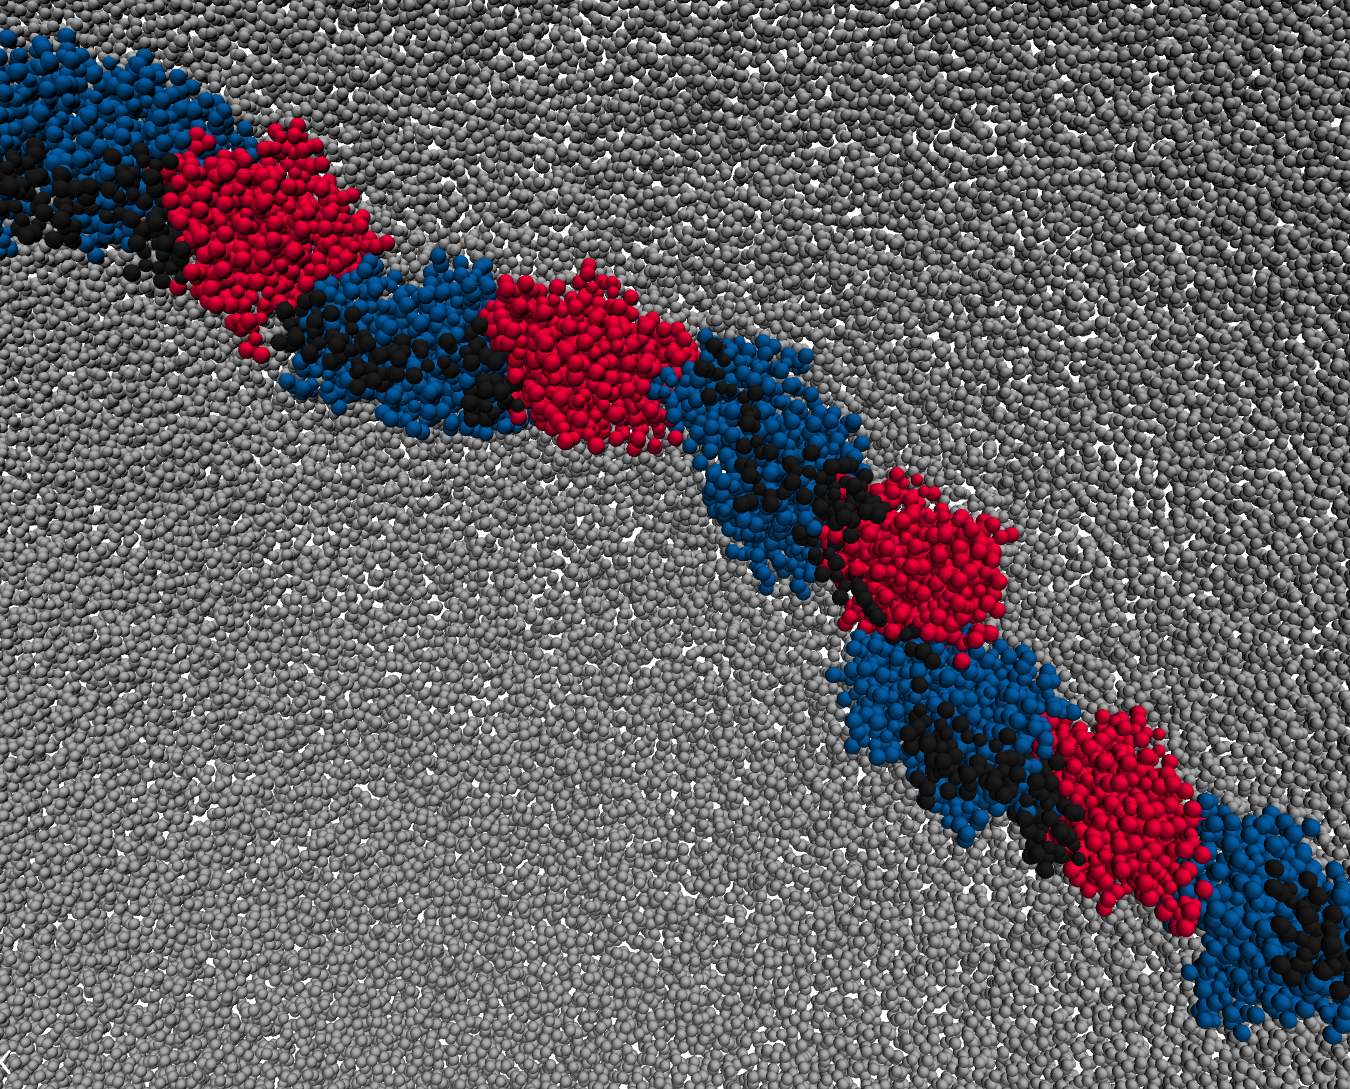
\includegraphics[height=3cm]{figures/results/fak_chainlike}
	}\hfill%
	\subcaptionbox{\label{clust:3d_ring}}[0.32\textwidth]{
		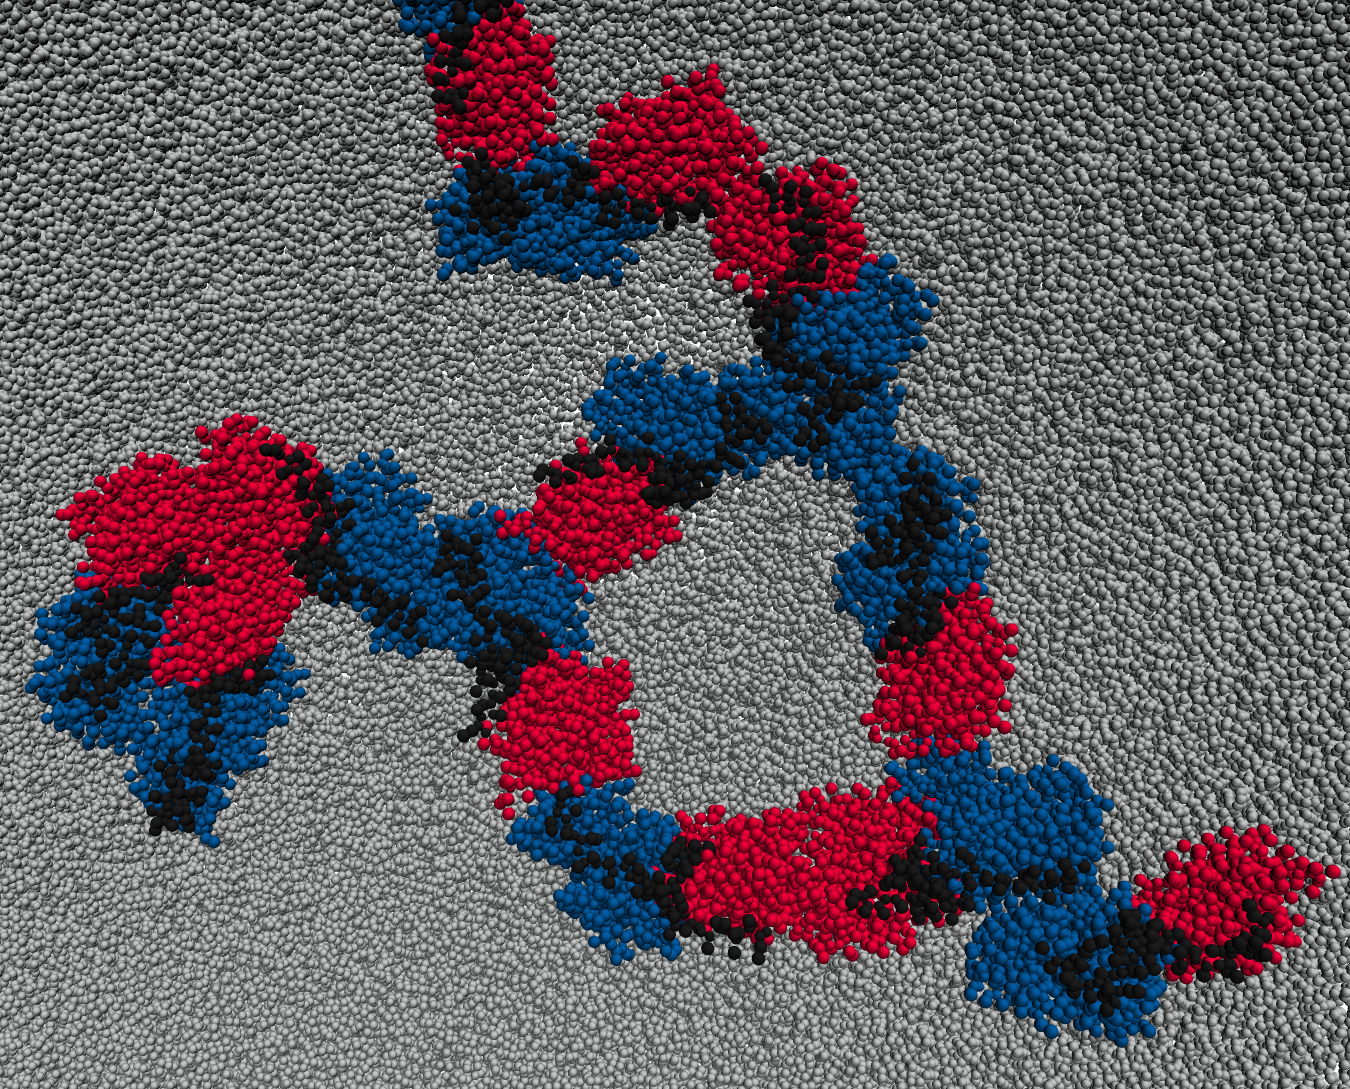
\includegraphics[height=3cm]{figures/results/fak_circle}
	}\hfill%
	\subcaptionbox{\label{clust:3d_aggl}}[0.32\textwidth]{
		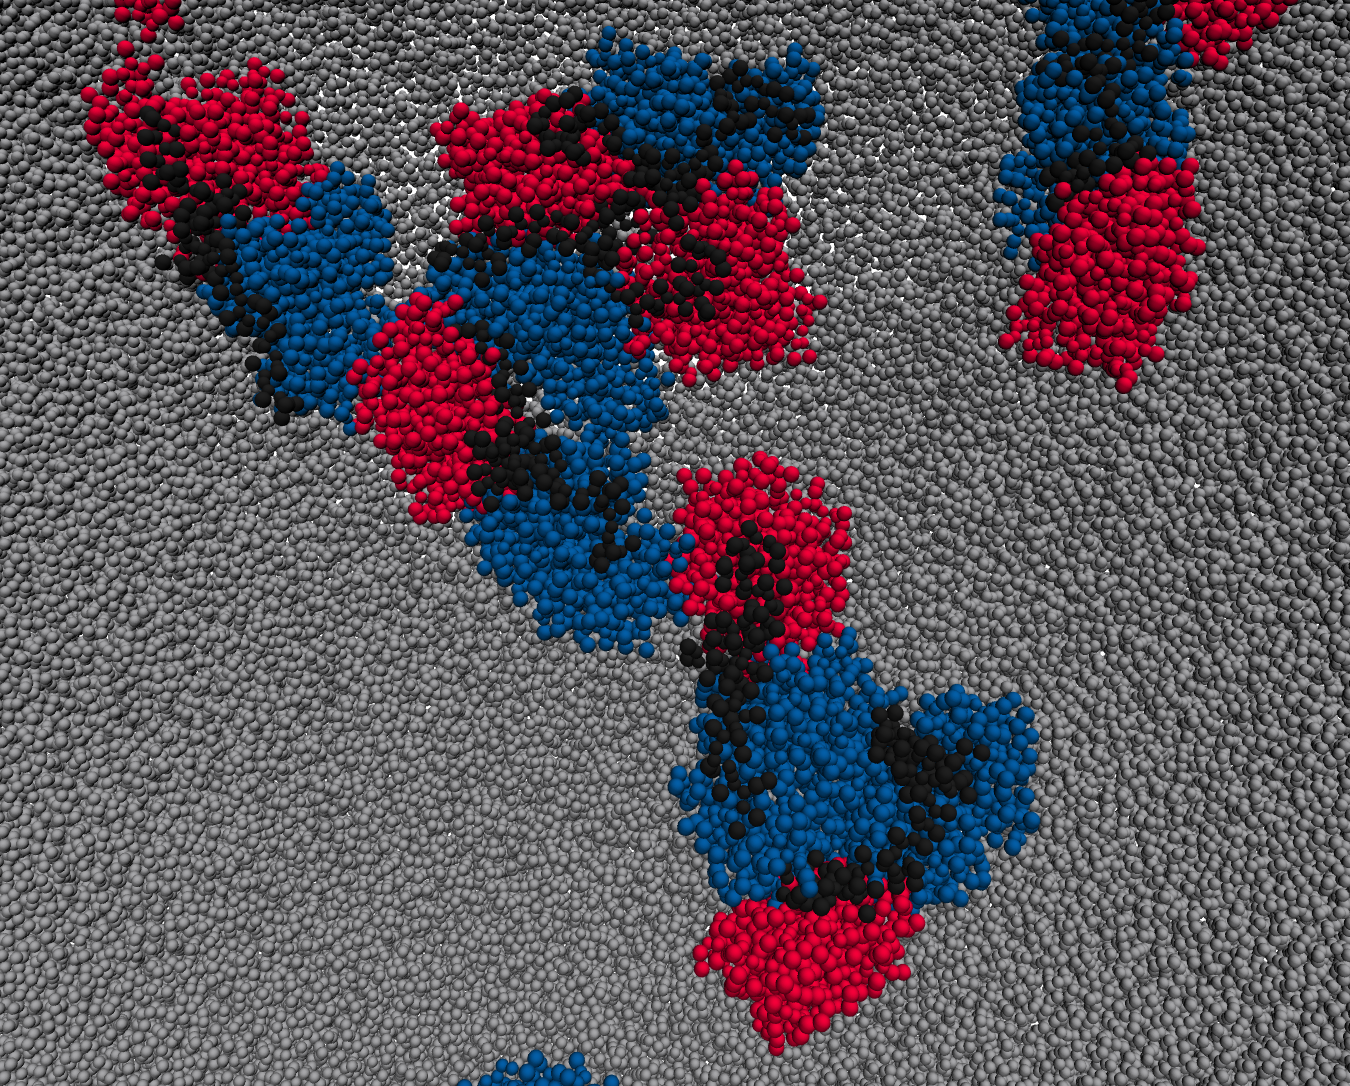
\includegraphics[height=3cm]{figures/results/fak_agglo}
	}
	\nicecaption{Obtained cluster shapes}{FAK molecules (FERM blue, kinase red, linker black) in different clusters on a membrane (grey). The shapes differ a lot and are hard to classify. Examples are chains (\subref{clust:3d_chain}), ring-like structures (\subref{clust:3d_ring}) and agglomerations (\subref{clust:3d_aggl})}
	\label{clust:3d}
\end{figure}
%
%
%
\\
In order to classify the occurring interactions, we analysed the time evolution of the neighbouring types as well as the transitions among them (see \autoref{mult:inttype_both}). These plots indicate that interactions involving two domains in total (type 1, 2 and 3) occur much more often than interactions involving four domains (type 6 and 7). Especially type 7 neighbours seem to be unstable, since they always lose contact immediately after the formation (see \autoref{mult:inttype_vs_t}, pink line). Therefore, a tendency for interactions along the long axis of FAK can be deduced.\\
Furthermore, the mean number of neighbours is considered. This quantity rises fast in the beginning and flattens after $6\,\si{\micro\second}$. The average over the five copies is $1.86$ neighbours at the end of the simulations.\\
From these observations, the conclusion can be drawn that the preferred arrangement of FAK molecules are chains along their long axis. The FAK molecules inside the chain can interact either as type 3 neighbours (FK chains) or as type 1 and type 2 neighbours (FFKK chains). Combinations of these two are also possible.
%
%
%
\begin{figure}
	\subcaptionbox{\label{mult:inttype_vs_t}}[0.49\textwidth]{
		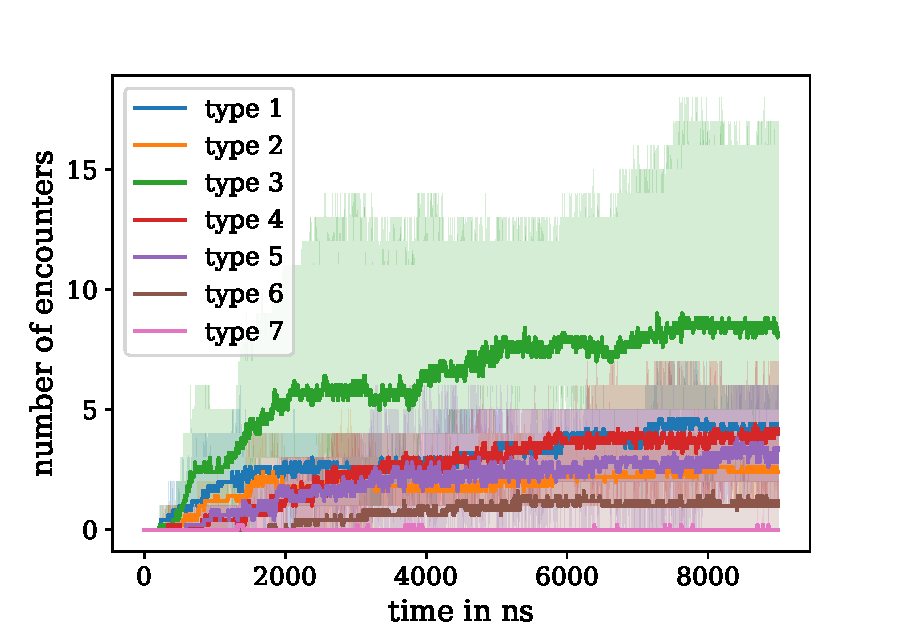
\includegraphics[height=5cm]{figures/results/multiple_typevstime}
	}\hfill%
	\subcaptionbox{\label{mult:inttype_markov}}[0.49\textwidth]{
		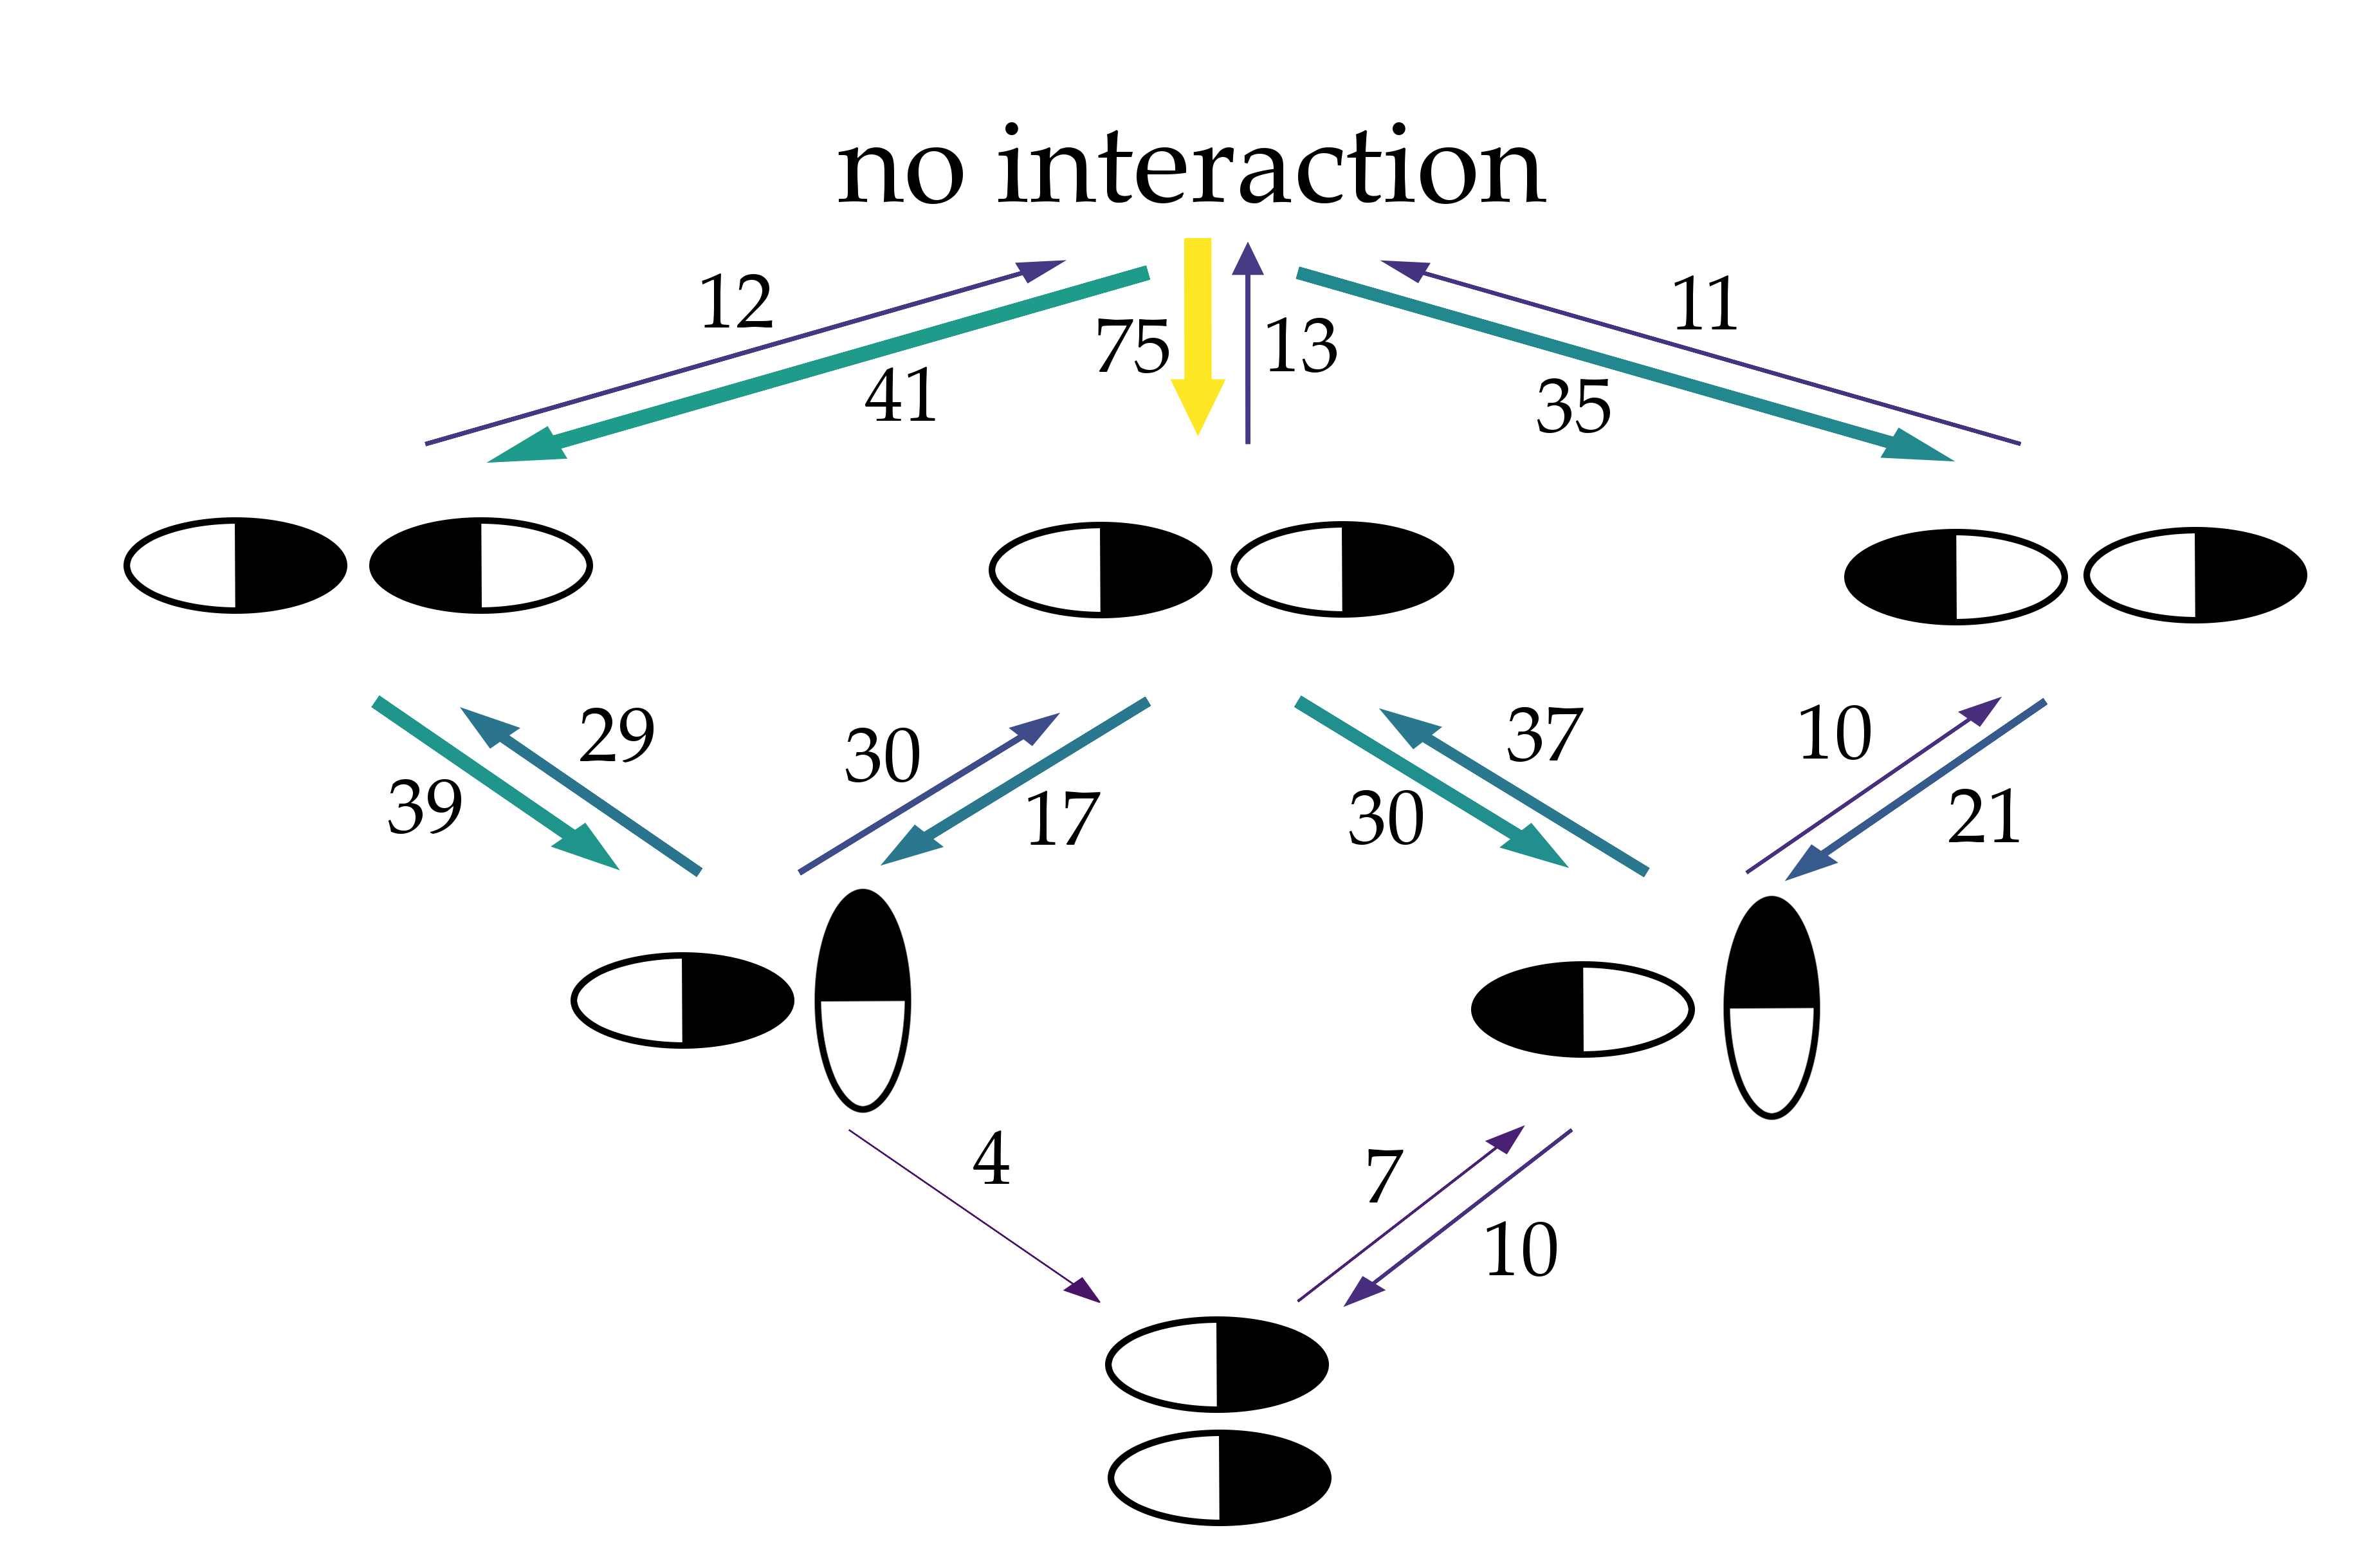
\includegraphics[height=5cm]{figures/results/markov}
	}%
	\nicecaption{Evolution of neighbouring types}{(\subref{mult:inttype_vs_t}): Mean number of encounters over the five copies for the different neighbouring types. The filled area shows the range from minimum to maximum. (\subref{mult:inttype_markov}): Transition diagram of the neighbouring types. Width and colour of the arrows correspond to the total number of observed transitions, which is also given beside the arrows. For simplicity, only transitions which occurred more than $5\%$ of the maximum (at least 4 times) are shown.}
	\label{mult:inttype_both}
\end{figure}
%
%
%
\subsection{Activation due to clustering}
Lastly, the impact of clustering on FAK activation is addressed. Since activation means the dissociation of the FERM domain from the kinase, we analysed our data with respect to the CA values, $d_\text{F1-N}$ and $d_\text{F2-C}$.\\
Unfortunately, in no FAK molecule did a full dissociation take place at any time. In addition, the CA values seem to be independent of the number of neighbours, the interaction type and the clustersize. Because only a small number of FAK molecules was put into the system and the clustering process was not finished at the end of the simulations, this does not mean that activation due to clustering is impossible. In the hope of seeing trends regarding to activation, a more detailed analysis for the different proteins was performed.\\
\\
Motivated from \autoref{mult:oligs}, we focus on FAK molecules inside chains. A FAK molecule can be seen as a chain member if it has exactly two neighbours and if these neighbours are not neighbours of one another. For FK chains, only type 3 interactions were allowed, for FFKK chains both, type 1 and type 2. We compare the results for FK chains and FFKK chains to FAK-MEM (see \autoref{mult:fk_ca} and \autoref{mult:ff_ca}, respectively).\\
\autoref{mult:fk_ca} indicates that an arrangement of FAK molecules to FK chains does not influence the mean value of CA. The distribution gets slightly sharper compared to FAK-MEM, which could imply a stabilisation of the interface. Not even the distributions of $d_\text{F1-N}$ and $d_\text{F2-C}$ differ noticeably from those obtained in FAK-MEM.\\
Neither does an arrangement into FFKK chains affects the value of CA (\autoref{mult:ff_ca}) significantly. However, the distribution of $d_\text{F1-N}$ indicates a trend to larger values in comparison to FAK-MEM, which are linked to a more open state of FAK.\\
\\
The filtering leads to a smaller sampling of the distributions of $d_\text{F1-N}$, $d_\text{F2-C}$ and CA. For example, for FFKK chains ca. $40\%$ of the underlying dataset ($21.7\,\si{\micro\second}$ of simulation time in total) comes from one FAK instance only. Therefore, the statistical significance of the obtained difference doubtful.
%
%
%
%\begin{figure}
%	\centering
%	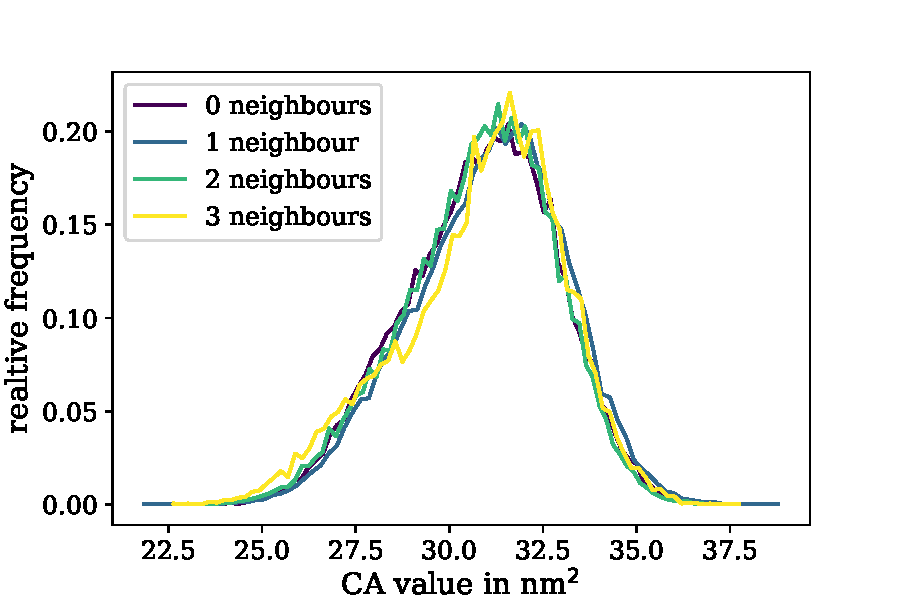
\includegraphics[height=5cm]{figures/results/nng_ca}
%	\nicecaption{CA for different numbers of neighbours}{}
%	\label{mult:nng_ca}
%\end{figure}
%
%
%
%
%
%
\begin{figure}[hb]
	\centering
	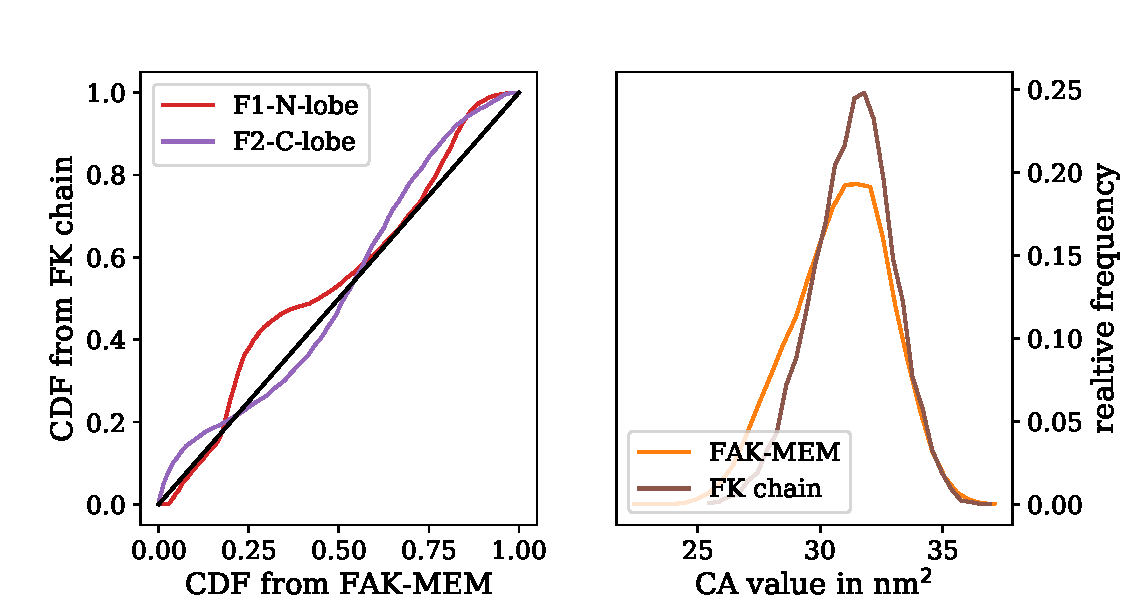
\includegraphics[height=6cm]{figures/results/fk_ca}
	\nicecaption{Domain distances and contact area of FK chains}{(left): The Q-Q plot of $d_\text{F1-N}$ and $d_\text{F2-C}$ distributions in comparison to FAK-MEM imply a strong similarity. (right): The CA value doesn't change noticeably in comparison to FAK-MEM.}
	\label{mult:fk_ca}
\end{figure}
%
%
%
%
%
%
%
\begin{figure}[t]
	\centering
	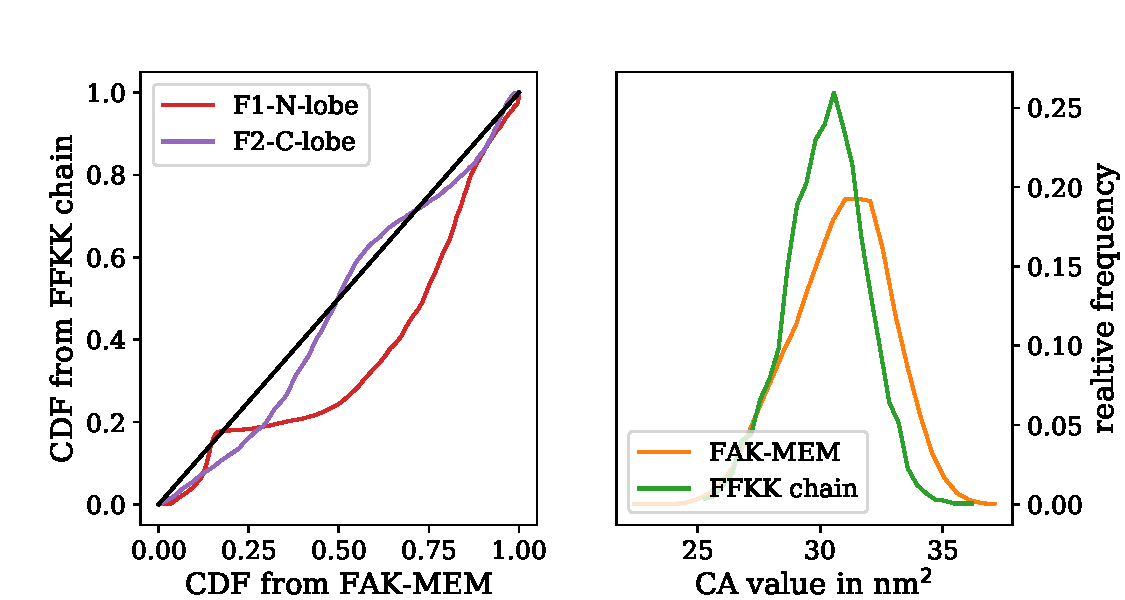
\includegraphics[height=6cm]{figures/results/ff_ca}
	\nicecaption{Domain distances and contact area of FFKK chains}{(left): The Q-Q plot of $d_\text{F1-N}$ and $d_\text{F2-C}$ distributions in comparison to FAK-MEM imply a tendency to larger distances of F1 and the N-lobe for FFKK chain members. (right): The CA value decreases slightly by $2\%.$.}
	\label{mult:ff_ca}
\end{figure}
%
%
%
%
